% -*- mode: noweb; noweb-default-code-mode: R-mode; -*-


% ------------------------------------------------------------------------
% bjourdoc.tex for birkjour.cls: Last revised April 3, 2021, by R.A.****
% ------------------------------------------------------------------------
%%%%%%%%%%%%%%%%%%%%%%%%%%%%%%%%%%%%%%%%%%%%%%%%%%%%%%%%%%%%%%%%%%%%%%%%%%

\documentclass{birkjour}
%%%Optional but convenient to use is the package ``cite''. If you do not want to use it, remark the next line by placing the percent sign % in front of it:
\usepackage[noadjust]{cite}
\usepackage{xcolor}
\usepackage{wrapfig}
\usepackage{amssymb}
\usepackage{Sweave}
\usepackage{doi}
\usepackage{url}
\RequirePackage[all]{xy}

%\include{Tmacros}

%
% THEOREM Environments (Examples)-----------------------------------------
%
\newtheorem{thm}{Theorem}[section]
\newtheorem{cor}[thm]{Corollary}
\newtheorem{lem}[thm]{Lemma}
\newtheorem{prop}[thm]{Proposition}
\theoremstyle{definition}
\newtheorem{defn}[thm]{Definition}
\theoremstyle{remark}
\newtheorem{rem}[thm]{Remark}
\newtheorem{comment}[thm]{Comment}
\newtheorem*{ex}{Example}
\numberwithin{equation}{section}
\newtheorem*{warning}{\textbf{Warning!}}


\newcommand{\BibTeX}{B\kern-0.1emi\kern-0.017emb\kern-0.15em\TeX}
\newcommand{\XYpic}{$\mathrm{X\kern-0.3em\raisebox{-0.18em}{Y}}$-$\mathrm{pic}\,$}
\newcommand{\TexnicCenter}{\TeX nicCenter}

%%%Clifford algebra macros
\newcommand{\cl}{C \kern -0.1em \ell}  %%Clifford algebra

\newcommand{\einf}{\mathbf{e}_\infty}
\newcommand{\ezero}{\mathbf{e}_0}



\DeclareMathOperator{\JJ}{\mathbin{\raisebox{0.25ex}%
                       {\mbox{\scriptsize$
                       \rm\vphantom{I}%
                       \_\hskip -0.25em\_%
                       \vrule width 0.6pt$}}}}           %left contraction

\DeclareMathOperator{\LL}{\mathbin{\raisebox{0.25ex}%
                        {\mbox{\scriptsize$
                        \rm\vphantom{I}%
                        \vrule width 0.6pt \hskip -0.5pt%
                        \_\hskip -0.25em\_$}}}}          %right contraction

\newcommand{\JJB}[1]{\JJ_{#1}}
\newcommand{\LLB}[1]{\LL_{#1}}


\newcommand{\w}{\wedge}
\newcommand{\bigw}{\bigwedge}
\newcommand{\dw}{\mathbin{\dot\wedge}}
\newcommand{\dwedge}{\mathbin{\dot\wedge}}

\DeclareMathOperator{\hotimes}{\Hat{\otimes}}
\DeclareMathOperator{\chr}{\mathrm{char}}

\newcommand{\bx}{\mathbf{x}}
\newcommand{\by}{\mathbf{y}}
\newcommand{\ba}{\mathbf{a}}
\newcommand{\bb}{\mathbf{b}}


%
\newcommand{\BF}{\mathbb{F}}
\newcommand{\BZ}{\mathbb{Z}}
\newcommand{\BR}{\mathbb{R}}
\newcommand{\BC}{\mathbb{C}}
\newcommand{\BH}{\mathbb{H}}

\newcommand{\ed}{\end{document}}
\begin{document}

%-------------------------------------------------------------------------
% editorial commands: to be inserted by the editorial office
%
%\firstpage{1} \volume{228} \Copyrightyear{2004} \DOI{003-0001}
%
%
%\seriesextra{Just an add-on}
%\seriesextraline{This is the Concrete Title of this Book\br H.E. R and S.T.C. W, Eds.}
%
% for journals:
%
%\firstpage{1}
%\issuenumber{1}
%\Volumeandyear{1 (2004)}
%\Copyrightyear{2004}
%\DOI{003-xxxx-y}
%\Signet
%\commby{inhouse}
%\submitted{March 14, 2003}
%\received{March 16, 2000}
%\revised{June 1, 2000}
%\accepted{July 22, 2000}
%
%
%
%---------------------------------------------------------------------------
%Insert here the title, affiliations and abstract:
%

\title[Clifford algebra in R]{
 Clifford algebra in R: introducing the {\tt clifford} package}
%----------Author 1
\author[Hankin]{Robin K. S. Hankin}
\address{%
  University of Stirling\\
  Stirling FK9 4LH\\
  United Kingdom
}
%
\email{hankin.robin@gmail.com}
%
%----------classification, keywords, date
\subjclass{Primary 15A66, 16W50, 20C05, 20C40, 20D15; Secondary 68W30}
%
\keywords{Class file, HTML, journal}
%
\date{\today}
%----------additions
\dedicatory{Last Revised:\\ \today}
%%% ----------------------------------------------------------------------
\begin{abstract}

Here I present the {\tt clifford} package for working with Clifford
algebras in the R programming language.  Algebras of arbitrary
dimension and signature can be manipulated, and a range of different
multiplication operators is provided.  The algebra is described and
package idiom is given; it obeys {\tt disordR} discipline.  The
package is available on CRAN and development versions are hosted at
github.


\end{abstract}
\label{page:firstblob}
%%% ----------------------------------------------------------------------
\maketitle
%%% ----------------------------------------------------------------------
\tableofcontents



\section{Introduction}

\setlength{\intextsep}{0pt}
\begin{wrapfigure}{r}{0.2\textwidth}
  \begin{center}
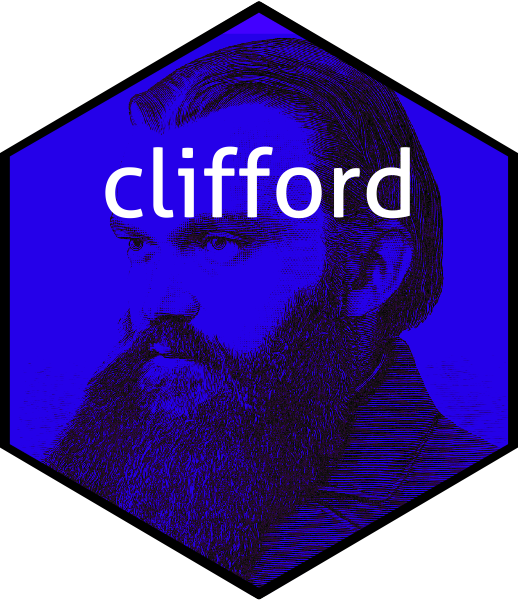
\includegraphics[width=1in]{clifford.png}
  \end{center}
\end{wrapfigure}
Clifford algebras~\cite{hestenes1987} are interesting and instructive
mathematical objects.  The class has a rich structure that has varied
applications to physics.  Computational support for working with the
Clifford algebras is part of a number of algebra systems including
Sage~\cite{sagemath2019} and \textit{sympy}~\cite{sympy2017}.  Here I
introduce the {\tt clifford} package, written in the R computing
language~\cite{rcore2022}, which furnishes functionality for working
with Clifford algebras.  The R language is easily
  augmented to manipulate symbolic mathematics and examples would
  include finite group theory~\cite{hankin2020_permutations}, Weyl
  algebra~\cite{hankin2022_weyl_arxiv}, and knot
  theory~\cite{hankin2023}.  As of 2024, no other R functionality for
  Clifford algebra is available.

Notation follows Snygg~\cite{snygg2010}.  The
package is available on CRAN at
\verb+https://CRAN.R-project.org/package=clifford+ and development
versions are hosted at github at
\verb+https://github.com/RobinHankin/clifford+.


\newcommand{\ei}[1]{\ensuremath{{\bf e}_{#1}}}


Suppose we consider $V=\mathbb{R}^n$, an $n$-dimensional vector space
spanned by basis vectors $\ei{1},\ldots,\ei{n}$.  Then an arbitrary
vector in this space will be $a^1\ei{1}+\cdots+a^n\ei{n}$.  The
associated Clifford algebra will be of dimension $2^n$, spanned by
formal products $\ei{i_1}\ei{i_2}\ldots\ei{i_r}$, $1\leqslant
i_1<\cdots<i_r\leqslant n$.  We write this as $\ei{i_1\ldots i_r}$ for
brevity.  The defining relations would be $\ei{i}\ei{j}=-\ei{j}\ei{i}$
for $i\neq j$ and

\begin{equation}\label{posdefcliff2}
\ei{i}\ei{i} = \begin{cases}
    +1, & \hphantom{p+{}}1\leqslant i\leqslant p\\
    -1, & \hphantom{p+{}}p < i\leqslant p+q\\
    0   & p+q < i\leqslant n.
  \end{cases}
\end{equation}

The Clifford algebra ${\mathcal C}_{p,q}$ (other notations include
$Cl(p,q)$) is then the algebra formed by $\mathbb{R}_{p,q}$ together
with formal products of basis vectors.  The value of
  $n$ is suppressed in this notation in much the same way as the
  length of a numeric vector is ignorable in base R; but is
  implemented---by way of option {\tt maxdim}---as a controllable
  option.  One special case would be $p=q=0$, implying that
$\ei{i}\ei{i}=0$ for $1\leqslant i\leqslant n$; geometric products
become wedge products.

\section{Computational implementation}

In standard Clifford terminology, a {\em blade} is a
  product of one-vectors (that is, members of $V$), and a {\em basis
    blade} is a product of basis vectors.

The package represents basis blades using dynamic bitset objects from
the {\tt boost} library~\cite{karlsson2005}.  A bitset emulates an
array of Boolean elements, but is optimized for space allocation and
access/modification times.  The set bits specify the basis blades
present in a term; using bitsets allows products to use fast Boolean
operators.  An object such as $\ei{2}\ei{5}\ei{7}$ [or $\ei{257}$]
will be a bitset with bits 2, 5, and 7 set [note the off-by-one
  issue].  More detail on the implementation of products is given in
Table~\ref{cliffprods}.  Dynamic objects are needed here as the number
of bits in the set is specified at runtime.  A {\tt clifford} object
is an element of a Clifford algebra; this is set of basis blades, each
with a real coefficient.  The {\tt stl} map class~\cite{musser2009} is
used:

{\ }\\[10pt]
\begin{verbatim}
typedef boost::dynamic_bitset<> blade;
typedef map<blade, long double> clifford;
\end{verbatim}

{\ }\\[10pt]

A ``map'' is a sorted associative container that contains key-value
pairs with unique keys~\cite{musser2009}.  A {\tt clifford} object
thus maps dynamic bitsets (basis blades) to coefficients, here long
doubles.  \textcolor{blue}{The {\tt STL map} class is used for
  efficiency: search, and insertion/deletion operations are
  consistently $\mathcal{O}(\log m)$, where $m$ is the number of
  nonzero coefficients.  For example, elements of any clifford algebra
  on $V=\mathbb{R}^n$ will have at most $2^n$ non-zero coefficients,
  searchable and manipulable in time $\mathcal{O}(n)$; further, any
  $k$-vector will have ${n\choose k}\lesssim 2^n/\sqrt{n}$ possible
  coefficients, so operations will again be $\mathcal{O}(n)$.  The
  various products presented in Table~\ref{cliffprods} are more
  complicated but the geometric product of two $k$-vectors will
  involve $\lesssim\mathcal{O}(4^n/n)$ (scalar) multiplications, and
  the outer product will involve $\lesssim\mathcal{O}(2^n/\sqrt{n})$
  multiplications.}  Similar techniques are used in the {\tt spray}
and {\tt mvp} packages~\cite{hankin2022_mvp,hankin2022_spray} which
furnish functionality for multivariate polynomials.




\section{Outline of the computational method}

A Clifford object is the formal sum of terms; a term is a basis blade
with an an associated coefficient; sums are managed by an STL map.
Scalar multiplication is distributive; addition is performed
elementwise via a standard container iterator.

The six ``ordinary'' products (that is, the first six products of
Table~\ref{cliffprods}) are implemented using a standardised system.
Distributivity means we only need consider the product of basis
blades.

To calculate the product of, say, $\ei{257}$ by $\ei{34}$, we first of
all count the intersection of the set bits in the ranges $1\leqslant
i\leqslant p$, $p<i\leqslant p+q$, and $i >p+q$ to determine whether a sign flip
is required or to set the product to zero.  The different types of
product have different rules for setting the product to zero (this is
a little difficult to see at first glance; but taking the outer
product as an example, $\displaystyle A\wedge
B=\sum_{r,s}\left\langle\left\langle A\right\rangle_r\left\langle
B\right\rangle_s\right\rangle_{s+r}$, we can see that any common set
bits in the basis blades of $A$ and $B$ will reduce the grade of their
product, thus by definition having non-empty intersection zeros the
product).  We then write the product by juxtaposing the set bits to
arrive at $\ei{25734}$; and then count the number of transpositions
required to sort the set bits an arrive at $\ei{23457}$.  The boost
library performs all these operations quickly and efficiently.  The
coefficient of the product is just the product of the coefficient,
modulo the sign.


\section{The package in use}

Suppose we specify that $\ei{i}\ei{i}=+1$,
  $i\geqslant 1$ (the default in the package) and want to work with
Clifford object $1+2\ei{1}+3\ei{2}+4\ei{2}\ei{3}$.  In R idiom this
would be

\begin{Schunk}
\begin{Sinput}
> (x <- 1 + 2*e(1) + 3*e(2) + 4*e(2:3))
\end{Sinput}
\begin{Soutput}
Element of a Clifford algebra, equal to
+ 1 + 2e_1 + 3e_2 + 4e_23
\end{Soutput}
\end{Schunk}

Here we have used function {\tt e()} which takes an integer vector
that specifies the term.  Note that the {\tt *}
  operator is ``overloaded''~\cite{stroustrup2013}: that is, it is
  sensitive to the class of object on either side, and in this case
  {\tt e(i)} is a Clifford object.  Addition and subtraction work as
expected:

\begin{Schunk}
\begin{Sinput}
> y <- e(1) + 55*e(1:5)
> x-y
\end{Sinput}
\begin{Soutput}
Element of a Clifford algebra, equal to
+ 1 + 1e_1 + 3e_2 + 4e_23 - 55e_12345
\end{Soutput}
\end{Schunk}

In the above, see how the $\ei{1}$ term has vanished.  We can
multiply Clifford elements using natural R idiom:
>
\begin{Schunk}
\begin{Sinput}
> x*x
\end{Sinput}
\begin{Soutput}
Element of a Clifford algebra, equal to
- 2 + 4e_1 + 6e_2 + 8e_23 + 16e_123
\end{Soutput}
\end{Schunk}

(Multiplication that Snygg denotes by juxtaposition is here indicated
with a {\tt *}).  We can consider arbitrarily high dimensional data:

\begin{Schunk}
\begin{Sinput}
> (z <- as.1vector(1:7))
\end{Sinput}
\begin{Soutput}
Element of a Clifford algebra, equal to
+ 1e_1 + 2e_2 + 3e_3 + 4e_4 + 5e_5 + 6e_6 + 7e_7
\end{Soutput}
\begin{Sinput}
> z*x
\end{Sinput}
\begin{Soutput}
Element of a Clifford algebra, equal to
+ 8 + 1e_1 - 10e_2 - 1e_12 + 11e_3 - 6e_13 - 9e_23 + 4e_123 +
4e_4 - 8e_14 - 12e_24 + 16e_234 + 5e_5 - 10e_15 - 15e_25 + 20e_235 +
6e_6 - 12e_16 - 18e_26 + 24e_236 + 7e_7 - 14e_17 - 21e_27 + 28e_237
\end{Soutput}
\end{Schunk}

In the above, we coerce a vector to a Clifford 1-vector.  The package
includes many functions to create elements of Clifford algebras,
including {\tt rcliff()}, a routine for generating
simple random Clifford objects with small integer
  coefficients:

\begin{Schunk}
\begin{Sinput}
> rcliff()
\end{Sinput}
\begin{Soutput}
Element of a Clifford algebra, equal to
+ 5 - 5e_1 - 1e_4 + 4e_24 + 3e_5 + 6e_6 - 2e_26 - 4e_36 - 3e_1246
\end{Soutput}
\end{Schunk}

The defaults for {\tt rcliff()} specify that the object is a sum of
grade-4 terms but this can be altered:

\begin{Schunk}
\begin{Sinput}
> (x <- rcliff(d=7,g=5,include.fewer=TRUE))
\end{Sinput}
\begin{Soutput}
Element of a Clifford algebra, equal to
+ 7 - 9e_3 - 7e_4 - 3e_1234 + 2e_6 + 1e_136 + 9e_1246 + 5e_456
+ 7e_1237 + 8e_13567
\end{Soutput}
\begin{Sinput}
> elements(grades(x))
\end{Sinput}
\begin{Soutput}
 [1] 0 1 1 4 1 3 4 3 4 5
\end{Soutput}
\end{Schunk}

Above, argument {\tt include.fewer} directs {\tt
    rcliff()} to return a Clifford object that includes terms with
  grades lower than the specified {\tt g=5}; on the next line, {\tt
    elements()} is needed to coerce the disord-compliant output of
  {\tt grades()} to a normal R vector; full details are given
  in~\cite{hankin2022_disordR}.

\section{Pseudo-Euclidean spaces}

The signature of the metric may be altered.  Starting with the
Euclidean case we have:
    
\begin{Schunk}
\begin{Sinput}
> e1 <- e(1)
> e2 <- e(2)
> e1*e1
\end{Sinput}
\begin{Soutput}
Element of a Clifford algebra, equal to
scalar ( 1 )
\end{Soutput}
\begin{Sinput}
> e2*e2
\end{Sinput}
\begin{Soutput}
Element of a Clifford algebra, equal to
scalar ( 1 )
\end{Soutput}
\end{Schunk}

However, if we wish to consider $p=1$, $q=1$ [thus
    $\ei{1}^2=+1$, $\ei{2}^2=-1$], package idiom is to use the {\tt
    signature()} function:

\begin{Schunk}
\begin{Sinput}
> signature(1,1)  # signature +-
> e1*e1 # as before, returns +1
\end{Sinput}
\begin{Soutput}
Element of a Clifford algebra, equal to
scalar ( 1 )
\end{Soutput}
\begin{Sinput}
> e2*e2 # should return -1
\end{Sinput}
\begin{Soutput}
Element of a Clifford algebra, equal to
scalar ( -1 )
\end{Soutput}
\end{Schunk}

Suppose we wish to use a signature $+++-$, corresponding to the
Minkowski metric in special relativity; this would be indicated in
package idiom by {\tt signature(3,1)}.  Note that the clifford objects
themselves do not store the signature; it is used only by the product
operation {\tt *}.

\begin{Schunk}
\begin{Sinput}
> x <- rcliff(d=4,g=3,include.fewer=TRUE)
> y <- rcliff(d=4,g=3,include.fewer=TRUE)
\end{Sinput}
\end{Schunk}

Then we may multiply these two clifford objects using either the
default positive-definite inner product, or the Minkowski metric:

\begin{Schunk}
\begin{Sinput}
> x*y
\end{Sinput}
\begin{Soutput}
Element of a Clifford algebra, equal to
+ 20 + 36e_1 - 92e_2 - 90e_12 + 37e_3 + 6e_13 + 92e_23 - 30e_123 -
10e_4 - 94e_24 - 22e_124 + 87e_34 + 29e_134 - 21e_234 - 20e_1234
\end{Soutput}
\begin{Sinput}
> signature(3,1)  # switch to signature +++-
> x*y
\end{Sinput}
\begin{Soutput}
Element of a Clifford algebra, equal to
+ 20 + 90e_1 - 56e_2 - 50e_12 - 38e_3 - 51e_13 + 106e_23 + 30e_123 +
2e_4 - 136e_24 - 40e_124 - 15e_34 + 15e_134 - 21e_234 - 20e_1234
\end{Soutput}
\end{Schunk}

In the above, see how the products are different using the two inner
products.  

\section{Grassmann algebra}

A Grassmann algebra corresponds to a Clifford algebra with identically
zero inner product.  Package idiom is to use a zero signature:

\begin{Schunk}
\begin{Sinput}
> signature(0,0)  # specify null inner product
\end{Sinput}
\end{Schunk}
\begin{Schunk}
\begin{Sinput}
> is.zero(e(5)^2)     # should be TRUE
\end{Sinput}
\begin{Soutput}
[1] TRUE
\end{Soutput}
\end{Schunk}

This is a somewhat clunky way of reproducing the functionality of the
{\tt stokes} package~\cite{hankin2022_stokes_arxiv}.  To create
example objects illustrating this feature of the package, we use {\tt
  clifford()}, the {\em formal} creation method for Clifford objects:

\begin{Schunk}
\begin{Sinput}
> (x <- clifford(list(1:3, c(2,3,7)), coeffs=3:4))
\end{Sinput}
\begin{Soutput}
Element of a Clifford algebra, equal to
+ 3e_123 + 4e_237
\end{Soutput}
\end{Schunk}

(above we see how {\tt clifford()} takes a list of basis blades and a
vector of coefficients).  We may take the wedge prduct of {\tt x} with
another object {\tt y}, created in the same way:

\begin{Schunk}
\begin{Sinput}
> y <- clifford(list(1:3, c(1,4,5), c(4,5,6)), coeffs=1:3)
> x %^% y
\end{Sinput}
\begin{Soutput}
Element of a Clifford algebra, equal to
+ 9e_123456 - 8e_123457 - 12e_234567
\end{Soutput}
\end{Schunk}

then the {\tt stokes} idiom for this would be:

\begin{Schunk}
\begin{Sinput}
> (x <- as.kform(rbind(1:3,c(2,3,7)),3:4))
\end{Sinput}
\begin{Soutput}
           val
 2 3 7  =    4
 1 2 3  =    3
\end{Soutput}
\begin{Sinput}
> (y <- as.kform(rbind(1:3,c(1,4,5),4:6),1:3))
\end{Sinput}
\begin{Soutput}
           val
 1 2 3  =    1
 1 4 5  =    2
 4 5 6  =    3
\end{Soutput}
\begin{Sinput}
> x %^% y
\end{Sinput}
\begin{Soutput}
                 val
 1 2 3 4 5 6  =    9
 2 3 4 5 6 7  =  -12
 1 2 3 4 5 7  =   -8
\end{Soutput}
\end{Schunk}


\section{Positive-definite inner product}

Function {\tt signature()} takes an infinite argument to make the
inner product positive-definite:

\begin{Schunk}
\begin{Sinput}
> signature(Inf)
\end{Sinput}
\end{Schunk}

(internally the package sets the signature to {\tt
  .Machine\$integer.max}, a near-infinite integer).  With this,
$\ei{i}\ei{i}=+1$ for any $i$.  For example, if
  $i=53$ we have:

\begin{Schunk}
\begin{Sinput}
> e(53)^2
\end{Sinput}
\begin{Soutput}
Element of a Clifford algebra, equal to
scalar ( 1 )
\end{Soutput}
\end{Schunk}


\section{Left and right contractions}

\cite{dorst2002} defines the left contraction $A\rfloor B$ and right
contraction $A\lfloor B$ (\cite{chisholm2012} calls these left and
right inner products) as follows:

\begin{eqnarray}
\displaystyle A\rfloor B = \sum_{r,s}\left\langle\left\langle
A\right\rangle_r\left\langle B\right\rangle_s\right\rangle_{s-r}\\
\displaystyle A\lfloor B = \sum_{r,s}\left\langle\left\langle
A\right\rangle_r\left\langle B\right\rangle_s\right\rangle_{r-s}
\end{eqnarray}

(it is understood that $n<0$ implies $\left\langle
  X\right\rangle_n=0$ for any Clifford object).
Package idiom for these would be {\tt A\%\_|\%B} and {\tt A\%|\_\%B}
---or {\tt lefttick(A,B)} and {\tt righttick(A,B)}---respectively.
Thus:

\begin{Schunk}
\begin{Sinput}
> (A <- rcliff())
\end{Sinput}
\begin{Soutput}
Element of a Clifford algebra, equal to
+ 7 - 9e_1 + 7e_2 - 5e_23 + 9e_123 + 5e_5 - 7e_15 + 2e_1456
\end{Soutput}
\begin{Sinput}
> (B <- rcliff())
\end{Sinput}
\begin{Soutput}
Element of a Clifford algebra, equal to
+ 6 - 2e_2 + 6e_3 - 7e_123 + 7e_14 - 3e_5 + 2e_26 + 1e_46 +
9e_2346 - 9e_256
\end{Soutput}
\begin{Sinput}
> A %_|% B
\end{Sinput}
\begin{Soutput}
Element of a Clifford algebra, equal to
+ 76 - 35e_1 - 14e_2 + 42e_3 + 49e_13 + 63e_23 - 49e_123 - 63e_4 +
49e_14 - 21e_5 + 14e_6 + 59e_26 + 52e_46 + 63e_346 + 63e_2346 -
63e_56 - 63e_256
\end{Soutput}
\begin{Sinput}
> A %|_% B
\end{Sinput}
\begin{Soutput}
Element of a Clifford algebra, equal to
+ 76 - 33e_1 + 12e_2 + 54e_12 - 10e_3 + 18e_13 - 30e_23 + 54e_123 +
30e_5 - 40e_15 + 6e_146 - 14e_56 + 12e_1456
\end{Soutput}
\end{Schunk}

One thing to be wary of is the order of operations.  Thus
$\ei{2}\rfloor\ei{12}=-\ei{1}$ (in a positive-definite space) but

\begin{Schunk}
\begin{Sinput}
> e(2) %_|% e(1)*e(2)
\end{Sinput}
\begin{Soutput}
Element of a Clifford algebra, equal to
the zero clifford element (0)
\end{Soutput}
\end{Schunk}

because this is parsed as $(\ei{2}\rfloor\ei{1})\ei{2}=0\ei{2}=0$.  To
evaluate this as intended we need to include brackets:

\begin{Schunk}
\begin{Sinput}
> e(2) %_|% (e(1)*e(2))
\end{Sinput}
\begin{Soutput}
Element of a Clifford algebra, equal to
- 1e_1
\end{Soutput}
\end{Schunk}

although in this case it might be preferable to create the terms directly:

\begin{Schunk}
\begin{Sinput}
> e(2) %_|% e(1:2)
\end{Sinput}
\begin{Soutput}
Element of a Clifford algebra, equal to
- 1e_1
\end{Soutput}
\end{Schunk}


\subsection{Numerical verification of left and right inner product identities}

Chisholm gives a number of identities for these products including

\begin{eqnarray}
  A\rfloor(B\lfloor C) &=& (A\rfloor B)\lfloor C\\
  A\rfloor(B\rfloor C) &=& (A\wedge B)\rfloor C\\
  A\lfloor(B\wedge  C) &=& (A\lfloor B)\lfloor C
\end{eqnarray}

In package idiom:

\begin{Schunk}
\begin{Sinput}
> A <- rcliff();  B <- rcliff();  C <- rcliff()
> A %_|% (B %|_% C) == (A %_|% B) %|_% C
\end{Sinput}
\begin{Soutput}
[1] TRUE
\end{Soutput}
\begin{Sinput}
> A %_|% (B %_|% C) == (A %^%  B) %_|% C
\end{Sinput}
\begin{Soutput}
[1] TRUE
\end{Soutput}
\begin{Sinput}
> A %|_% (B %^%  C) == (A %|_% B) %|_% C
\end{Sinput}
\begin{Soutput}
[1] TRUE
\end{Soutput}
\end{Schunk}
\section{Higher dimensional spaces}

Ab\l{}amowicz and Fauser~\cite{ablamowicz2012} consider
high-dimensional Clifford algebras and consider the following two
elements of the 1024-dimensional Clifford algebra which we may treat
as ${\mathcal C}_{7,3}$ spanned by $\ei{1},\ldots,\ei{10}$ and perform
a calculation which I reproduce below (although these authors
exploited Bott periodicity, a feature not considered here).

Firstly we change the default print method slightly:

\begin{Schunk}
\begin{Sinput}
> options("basissep" = ",")
\end{Sinput}
\end{Schunk}

(this separates the subscripts of the basis vectors with a comma,
which is useful for clarity if $n>9$).  We then define clifford
elements $x,y$:

\begin{Schunk}
\begin{Sinput}
> (x <- clifford(list(1:3,c(1,5,7,8,10)),c(4,-10)) + 2)
\end{Sinput}
\begin{Soutput}
Element of a Clifford algebra, equal to
+ 2 + 4e_1,2,3 - 10e_1,5,7,8,10
\end{Soutput}
\begin{Sinput}
> (y <- clifford(list(c(1,2,3,7),c(1,5,6,8),c(1,4,6,7)),c(4,1,-3)) - 1)
\end{Sinput}
\begin{Soutput}
Element of a Clifford algebra, equal to
- 1 + 4e_1,2,3,7 - 3e_1,4,6,7 + 1e_1,5,6,8
\end{Soutput}
\end{Schunk}

Their geometric product is given in the package as

\begin{Schunk}
\begin{Sinput}
> signature(7)
> x*y
\end{Sinput}
\begin{Soutput}
Element of a Clifford algebra, equal to
- 2 - 4e_1,2,3 - 16e_7 + 8e_1,2,3,7 - 6e_1,4,6,7 - 12e_2,3,4,6,7 +
2e_1,5,6,8 + 4e_2,3,5,6,8 - 40e_2,3,5,8,10 - 30e_4,5,6,8,10 +
10e_1,5,7,8,10
\end{Soutput}
\end{Schunk}

in agreement with \cite{ablamowicz2012}, although the terms appear in
a different order.


\section{\textcolor{blue}{Case study: spheres in conformal geometric algebra}}

\textcolor{blue}{
Perwass~\cite{perwass2009} shows that geometric entities such as
circles and spheres in $\mathbb{R}^3$ may be represented as points in
a conformal geometric algebra.  To use the package, we consider the
three Euclidean basis vectors $\mathbf{e}_1$, $\mathbf{e}_2$,
$\mathbf{e}_3$ together with two additional basis vectors
$\mathbf{e}_+$ and $\mathbf{e}_-$ obeying $\mathbf{e}_+^2=1$,
$\mathbf{e}_-^2=-1$, $\mathbf{e}_+\cdot\mathbf{e}_-=0$.
Hildenbrand~\cite{hildenbrand2013}
defines~$\ezero=\left(\mathbf{e}_--\mathbf{e}_+\right)/2$
and~$\einf=\mathbf{e}_- +\mathbf{e}_+$, representing ``the origin''
and ``the point at infinity'' respectively.  It is straightforward to
implement these objects using the package:}
\begin{Schunk}
\begin{Sinput}
signature(4,1)
eplus <- e(4)
eminus <- e(5)
e0 <- (eminus - eplus)/2
einf <- eminus + eplus
\end{Sinput}
\end{Schunk}
%
\textcolor{blue}{
Above we use package idiom to specify $\cl(4,1)$ with Euclidean basis
vectors $\mathtt{e(1),e(2),e(3)}$, and define conformal objects $e_+,
e_-, e_0,e_\infty$ in terms of {\tt e(4)} and {\tt e(5)}.  Perwass
shows that a point $\bx=(x_1,x_2,x_3)$ may be projectively extended to
$P\in\cl(4,1)$ by the expression $P = \bx+(\bx\cdot\bx)\einf/2
+\ezero$.  Package idiom for this is straightforward:}
\begin{Schunk}
\begin{Sinput}
point <- function(x){as.1vector(x) + sum(x^2)*einf/2 + e0}
point(c(5, -4, 7))
\end{Sinput}
\begin{Soutput}
Element of a Clifford algebra, equal to
+ 5e_1 - 4e_2 + 7e_3 + 44.5e_4 + 45.5e_5
\end{Soutput}
\end{Schunk}
%
\textcolor{blue}{
Perwass goes on to show that a sphere $S$ may be specified in terms of
four (conformal) points that lie on it:
%
\begin{equation}
  S = P_1\wedge P_2\wedge P_3\wedge P_4/ I
\end{equation}
%
where the $P_i$ are points that lie on the sphere and $I$ is the unit
pseudoscalar.  Here I demonstrate the package's capabilities by
finding the unique sphere that passes through four points.  This is
possible, but difficult, using standard Euclidean methods; but is a
one-liner in conformal geometry.  Below, I specify the center and
radius of a sphere in $\mathbb{R}^3$, choose four points on the
sphere, and numerically reconstruct the center and radius from the
resulting conformal sphere:}
%
\begin{Schunk}
\begin{Sinput}
center <- c(3, -5, 6)
radius <- 3
point_on_sphere  <- function(center, radius, vec){
  point(center + radius*vec/sqrt(sum(vec^2)))
}

p1 <- point_on_sphere(center, radius, c(1, 4, 2))
p2 <- point_on_sphere(center, radius, c(6,-5, 3))
p3 <- point_on_sphere(center, radius, c(0, 4, 0))
p4 <- point_on_sphere(center, radius, c(1, 0, 0))

S <- p1 ^ p2 ^ p3 ^ p4 / pseudoscalar()            
\end{Sinput}
\end{Schunk}
%
\textcolor{blue}{
Then we extract the radius and center and compare with the known
values of $3$ and $(3,-5,6)$ respectively.  The radius $r$ is given by
$r^2 = \left(\frac{S}{-S\cdot\einf}\right)^2$ and the center by
scaling the sandwich product $S\einf S$.}

\begin{Schunk}
\begin{Sinput}
> sqrt(drop((S / drop(S %.% einf))^2))
\end{Sinput}
\begin{Soutput}
[1]  3
\end{Soutput}
\begin{Sinput}
S_sandwich <- S * einf * S 
scaling_factor <- -zap(S_sandwich %.% (e(4) + e(5)))
getcoeffs(zap(S_sandwich / scaling_factor), 1:3)
\end{Sinput}
\begin{Soutput}
[1]  3 -5 6
\end{Soutput}
\end{Schunk}
%
\textcolor{blue}{
Above, we use function {\tt zap()} which cancels small coefficients
which appear due to numerical error; apart from that, we see that the
radius and center of the original sphere are reconstituted accurately
and efficiently, using natural R idiom.}

\section{Conclusions and further work}

The {\tt clifford} package furnishes a consistent and documented suite
of reasonably efficient {\tt R}-centric functionality.  The package is
available on CRAN at
\verb+https://CRAN.R-project.org/package=clifford+ and development
versions are hosted at github at
\verb+https://github.com/RobinHankin/clifford+.  Further work might
include implementation of spinor algebra (via
  existing R-centric symbolic matrix
  functionality~\cite{hankin2023_jordan,hankin2006_onion}), or perhaps
  a more complete implementation of Clifford inverses as introduced
  in~\cite{hitzer2017}.



\bibliographystyle{plain}
\bibliography{clifford}

\appendix
\section{Products and conjugations implemented in the package}


The package implements a number of products and involutions.  The
products are given in table~\ref{cliffprods}.
  An involution is a function that is its own inverse, or
  equivalently ${f(f(x))=x}$.  There are several important
  involutions on Clifford objects; these commute past the grade operator
  with ${f(\left\langle A\right\rangle_r)=\left\langle
  f(A)\right\rangle_r}$ and are linear: ${f(\alpha A+\beta
  B)=\alpha f(A)+\beta f(B)}$.\\
  The dual is documented here for convenience, even though it is
  not an involution (applying the dual \emph{four} times is the
  identity).
  \itemize{
    \item The {\bf reverse} ${A^\sim}$ is given by {\tt rev()} (both Perwass
      and Dorst use a tilde, as in ${\tilde{A}}$ or ${A^\sim}$.
      However, both Hestenes and Chisholm use a dagger, as in
      ${A^\dagger}$.  Here, I use Perwass's notation).  The reverse of
      a term written as a product of basis vectors is simply the
      product of the same basis vectors but written in reverse order.
      This changes the sign of the term if the number of basis vectors
      is 2 or 3 (modulo 4).  Thus, for example,
      ${\left(e_1e_2e_3\right)^\sim=e_3e_2e_1=-e_1e_2e_3}$ and
      ${\left(e_1e_2e_3e_4\right)^\sim=e_4e_3e_2e_1=+e_1e_2e_3e_4}$.
      Formally, if ${X=e_{i_1}\ldots e_{i_k}}$, then
      ${\tilde{X}=e_{i_k}\ldots e_{i_1}}$.
        $$
        {\left\langle
          A^\sim\right\rangle_r=\widetilde{\left\langle
	    A\right\rangle_r}=(-1)^{r(r-1)/2}\left\langle A\right\rangle_r}
          $$
    Perwass shows that ${\left\langle
      AB\right\rangle_r=(-1)^{r(r-1)/2}\left\langle\tilde{B}\tilde{A}\right\rangle_r}$.
    \item The {\bf Conjugate} ${A^\dagger}$ is given by
    {\tt Conj()} (we use Perwass's notation, def 2.9 p59).  This
    depends on the signature of the Clifford algebra; see
    {\tt grade.Rd} for notation.  Given a basis blade
    ${e_\mathbb{A}}$ with ${\mathbb{A}\subseteq\left\lbrace
    1,\ldots,p+q\right\rbrace}$, then we have
    ${e_\mathbb{A}^\dagger = (-1)^m {e_\mathbb{A}}^\sim}$,
    where ${m=\mathrm{gr}_{-}(\mathbb{A})}$.  Alternatively,
    we might say
    $$
    {\left(\left\langle
    A\right\rangle_r\right)^\dagger=(-1)^m(-1)^{r(r-1)/2}\left\langle
    A\right\rangle_r }
    $$
    where
    ${m=\mathrm{gr}_{-}(\left\langle A\right\rangle_r)}$ [NB
    I have changed Perwass's notation].
    \item The {\bf main (grade) involution} or {\bf grade involution}
    ${\widehat{A}}$ is given by {\tt gradeinv()}.  This
    changes the sign of any term with odd grade:
    $$
    {\widehat{\left\langle A\right\rangle_r} =(-1)^r\left\langle
      A\right\rangle_r}
    $$
    (I don't see this in Perwass or Hestenes; notation follows Hitzer
    and Sangwine).  It is a special case of grade negation.
    \item The {\ bf grade ${r}$-negation} ${A_{\overline{r}}}$ is
      given by {\tt neg()}.  This changes the sign of the grade ${r}$
      component of ${A}$.  It is formally defined as ${A-2\left\langle
        A\right\rangle_r}$ but function {\tt neg()} uses a more
      efficient method.  It is possible to negate all terms with
      specified grades, so for example we might have ${\left\langle
        A\right\rangle_{\overline{\left\lbrace 1,2,5\right\rbrace}} =
        A-2\left( \left\langle A\right\rangle_1 +\left\langle
        A\right\rangle_2+\left\langle A\right\rangle_5\right)}$ and
      the R idiom would be {\tt neg(A,c(1,2,5))}.  Note that Hestenes
      uses ``${A_{\overline{r}}}$'' to mean the same as
      ${\left\langle A\right\rangle_r}$.
    \item The {\bf Clifford conjugate} ${\overline{A}}$ is given by
      {\tt cliffconj()}.  It is distinct from conjugation
      ${A^\dagger}$, and is defined in Hitzer and Sangwine as
    $$
    {\overline{\left\langle A\right\rangle_r} =
      (-1)^{r(r+1)/2}\left\langle A\right\rangle_r.}
    $$
    \item The {\bf dual} ${C^*}$ of a clifford object ${C}$ is given
      by {\tt dual(C,n)}; argument {\tt n} is the dimension of the
      underlying vector space.  Perwass gives ${C^*=CI^{-1}}$ where
      ${I=e_1e_2\ldots e_n}$ is the unit pseudoscalar [note that
        Hestenes uses ${I}$ to mean something different].  The dual is
      sensitive to the signature of the Clifford algebra \emph{and}
      the dimension of the underlying vector space.
      }

  
\begin{table}
  \begin{center}
    \begin{tabular}{lll}
        \hline\\
  Geometric product  & {\tt A*B = geoprod(A,B)}  &  $\displaystyle AB=\sum_{r,s}\left\langle A\right\rangle_r\left\langle B\right\rangle_s$ \\
    Inner product    & {\tt A \%.\% B = cliffdotprod(A,B)} &    $\displaystyle A\cdot B=\sum_{r\neq 0\atop s\ne 0}^{\vphantom{s\neq 0}}\left\langle\left\langle A\right\rangle_r\left\langle B\right\rangle_s\right\rangle_{\left|s-r\right|}$\\
    Outer product    &{\tt A \%\string^\% B = wedge(A,B)} &    $\displaystyle A\wedge B=\sum_{r,s}\left\langle\left\langle A\right\rangle_r\left\langle B\right\rangle_s\right\rangle_{s+r}$\\
    Fat dot product  &{\tt A \%o\% B = fatdot(A,B)} &  $\displaystyle A\bullet B=\sum_{r,s}\left\langle\left\langle A\right\rangle_r\left\langle B\right\rangle_s\right\rangle_{\left|s-r\right|}$\\
    Left contraction &{\tt A \%\_|\% B = lefttick(A,B)} & $\displaystyle A\rfloor B=\sum_{r,s}\left\langle\left\langle A\right\rangle_r\left\langle B\right\rangle_s\right\rangle_{s-r}$\\
    Right contraction &{\tt A \%|\_\% B = righttick(A,B)} & $\displaystyle A\lfloor B=\sum_{r,s}\left\langle\left\langle A\right\rangle_r\left\langle B\right\rangle_s\right\rangle_{r-s}$\\
    Cross product &{\tt A \%X\% B = cross(A,B)} &  $\displaystyle A\times B=\frac{1}{2_{\vphantom{j}}}\left(AB-BA\right)$\\
    Scalar product &{\tt A \%star\% B = star(A,B)} & $\displaystyle A\ast B=\sum_{r,s}\left\langle\left\langle A\right\rangle_r\left\langle B\right\rangle_s\right\rangle_0$\\
    Euclidean product &{\tt A \%euc\% B = eucprod(A,B)} &  $\displaystyle A\star B= A\ast B^\dagger$\\
    \hline
    \end{tabular}
  \end{center}
  \caption{\rule{0mm}{10mm} The Clifford products implemented in the\label{cliffprods} package}
  \end{table}

\section{Note on {\tt disordR} discipline}

Clifford objects are considered to be the sum of a finite number of
blades, each multiplied by a coefficient.  As discussed above, the
mapping itself is implemented using the {\tt STL} map
class~\cite{musser2009}; one reason why the this is fast is that the
order in which the key-value pairs are stored is undefined: the
compiler may store them in the order which it regards as most
propitious.  The order of storage is immaterial algebraically, as
addition is commutative and associative.  In the {\tt clifford}
package, the map is from blades to their coefficient, a real number.

However, one issue arising from the use of the {\tt map} class in
computational algebra is that the order of coefficients is
implementation-specific.  This can be problematic if one attempts to
access coefficients using standard vector notation, for the result is
not well-defined.  An example might be Clifford object
$3+4\ei{1}-5\ei{123}$ and its representation in the following R
session:

\begin{Schunk}
\begin{Sinput}
> p <- 3 + 4*e(1) - 5*e(1:3)
> p
\end{Sinput}
\begin{Soutput}
Element of a Clifford algebra, equal to
+ 3 + 4e_1 - 5e_123
\end{Soutput}
\end{Schunk}

We observe that {\tt p} is algebraically equivalent to
$4\ei{1}-5\ei{123}+3$ [the terms are written in a different order] and
the internal {\tt map} equivalent leverages this ambiguity by storing
the key-value pairs in whatever order the compiler finds most
propitious.  We might wish to extract the coefficients:

\begin{Schunk}
\begin{Sinput}
> coeffs(p)
\end{Sinput}
\begin{Soutput}
  A disord object with hash cb6600d951d6a0e1a666fb9217a896b7706ee3b5 and elements
[1]  3  4 -5
(in some order)
\end{Soutput}
\end{Schunk}

We see that the coefficients are $3,4,-5$, but the returned value---an
object of class {\tt disord}---declines to specify an order for these
coefficients.  This is because the order is implementation-specific,
and {\tt disordR} discipline will not ``guess'' which order is
actually employed.  For example, if we try to extract the first
element, an error is returned:

\begin{Schunk}
\begin{Sinput}
> p[1]
\end{Sinput}
\begin{Soutput}
Error in .local(x, i, j = j, ..., drop) : 
   if using a regular index to extract, must extract each
   element once and once only (or none of them)
> 
\end{Soutput}
\end{Schunk}

We see that the package refuses to declare which entry is the first,
and returns an error message.  Even though the order of coefficients
is not well defined, various statistics can be obtained:

\begin{Schunk}
\begin{Sinput}
> sum(coeffs(p))
\end{Sinput}
\begin{Soutput}
[1]  2
\end{Soutput}
\end{Schunk}

Here we observe that the sum of the coefficients {\em is} well
defined, whatever order is used for the summation: addition is
commutative and associative.  The {\tt disordR} package manages these
issues, essentially ensuring that meaningful questions with a
well-defined answer (such as the sum of coefficients) are executed
transparently and efficiently, while ill-posed questions with
implementation-specific results (such as the ``first'' element) return
an error.  The map class is used in a wide range of algebraic contexts
and {\tt disordR} discipline is enforced in a number of packages;
examples would
include~\cite{hankin2017_hyper2,hankin2023_frab,hankin2024_evitaicossa}.
Full details and further motivating examples are given
in~\cite{hankin2022_disordR}.

\end{document}
